\documentclass[12pt]{article}
\usepackage{fullpage}
\usepackage{titlesec}
\usepackage{tikz}
\usepackage{amsfonts,amssymb}
\usepackage{amsmath}
\usepackage{comment}
\usetikzlibrary{automata, positioning}

\input ../libraries/mac.tex
\input ../libraries/mathmac.tex

\begin{document}
\pagestyle{plain}
\titleformat{\subsection}[runin]
  {\normalfont\large\bfseries}{\thesubsection}{1em}{}

\title{Homework 4}
\author{Brooke Fugate, Michael O'Connor, Rohan Shah}
\date{}

\maketitle

\section*{Problem B5}
\subsection*{i.}
$M = (K, \Sigma, \Delta, \lambda, q_0, F)$ where $K = F = \{q_0\}$,
$\Sigma = \Delta = \{a,b\}$ and we can define $\lambda$ by induction on the
length of words $u\in \Sigma^*$ and $v \in \Delta^*$ such that $|u|=|v|$,
$(q_0, \epsilon, \epsilon, q_0) \in \lambda$ is the base case and by induction
if $(q_0, u, v, q_0) \in \lambda$ then $(q_0,au,bv,q_0), (q_0,bu,av,q_0) \in
\lambda$. A figure that illustrates
the a-transducer $M$ is:
\begin{center}
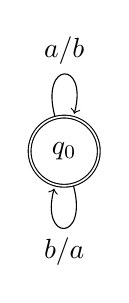
\begin{tikzpicture}[shorten >=1pt, node distance=2.5cm, on grid, auto]
  \node[state, accepting] (q0) {$q_0$};
  \path[->]
(q0) edge [loop above] node {$a/b$} (q0)
(q0) edge [loop below] node {$b/a$} (q0)
  ;
\end{tikzpicture}
\end{center}
\subsection*{ii.}

\subsection*{iii.}

\subsection*{iv.}

\subsection*{v.}

\end{document}
